\documentclass[10pt]{article}
\newcommand{\DIGESTDATE}{27 July 2026}
% ===================== PM Research Watch - shared preamble =====================
\usepackage[T1]{fontenc}
\usepackage[utf8]{inputenc}
\usepackage{amsmath,amssymb}
\usepackage{tgpagella}
\usepackage{tgheros}
\renewcommand{\sfdefault}{qhv}
\renewcommand{\ttdefault}{lmtt}
\usepackage{microtype}
\usepackage[english]{babel}

\usepackage[a4paper,top=17mm,bottom=17mm,left=17mm,right=17mm,
            headsep=6mm,footskip=10mm]{geometry}
\usepackage{graphicx}
\usepackage{xcolor}
\usepackage{colortbl}
\usepackage{tikz}
\usetikzlibrary{calc}
\usepackage[most]{tcolorbox}
\usepackage{titlesec}
\usepackage{fancyhdr}
\usepackage{booktabs}
\usepackage{array}
\usepackage{longtable}
\usepackage{enumitem}
\usepackage{multicol}
\usepackage{ragged2e}
\usepackage[hidelinks]{hyperref}

% ------------------------------------------------------------------ palette
\definecolor{Ink}    {HTML}{14262E}
\definecolor{Deep}   {HTML}{0F4C5C}
\definecolor{Teal}   {HTML}{1F7A8C}
\definecolor{Sky}    {HTML}{4FA3C4}
\definecolor{Sage}   {HTML}{6FA287}
\definecolor{Amber}  {HTML}{E3A008}
\definecolor{Clay}   {HTML}{B5643C}
\definecolor{Coral}  {HTML}{D1495B}
\definecolor{Violet} {HTML}{6A5B9E}
\definecolor{Slate}  {HTML}{4A6572}
\definecolor{Paper}  {HTML}{FBF9F5}
\definecolor{Mist}   {HTML}{EEEAE2}
\definecolor{Rule}   {HTML}{D9D3C9}

\pagecolor{Paper}
\color{Ink}

\hypersetup{colorlinks=true, linkcolor=Deep, urlcolor=Teal, citecolor=Teal,
            pdftitle={PM Research Watch}, pdfauthor={Automated daily digest}}

% ------------------------------------------------------------------ headings
\titleformat{\section}
  {\sffamily\bfseries\large\color{Deep}}{}{0pt}
  {}[{\vspace{1.2mm}\color{Amber}\titlerule[1.1pt]}]
\titlespacing*{\section}{0pt}{5.5mm}{2.8mm}

\titleformat{\subsection}
  {\sffamily\bfseries\normalsize\color{Teal}}{}{0pt}{}
\titlespacing*{\subsection}{0pt}{3.6mm}{1.4mm}

\setlist[itemize]{leftmargin=4.2mm, itemsep=1.1mm, topsep=1.3mm, parsep=0pt,
                  label=\textcolor{Teal}{\footnotesize$\blacktriangleright$}}

% ------------------------------------------------------------------ header/footer
\pagestyle{fancy}
\fancyhf{}
\renewcommand{\headrulewidth}{0pt}
\renewcommand{\footrulewidth}{0pt}
\fancyhead[L]{\sffamily\scriptsize\color{Slate}PM RESEARCH WATCH\;\textcolor{Rule}{\textbar}\;\DIGESTDATE}
\fancyhead[R]{\sffamily\scriptsize\color{Slate}Particulate matter monitoring \& health effects}
\fancyfoot[C]{\sffamily\scriptsize\color{Slate}\thepage}

% ------------------------------------------------------------------ components
% metric tile
\newcommand{\metric}[3]{%
  \begin{tcolorbox}[enhanced, colback=white, colframe=Rule, boxrule=0.5pt,
    arc=1.6mm, left=2.2mm, right=2.2mm, top=1.8mm, bottom=1.8mm,
    borderline west={1.7mm}{0pt}{#3}, nobeforeafter, valign=center,
    height=17mm, width=\linewidth]
    \RaggedRight
    {\sffamily\bfseries\fontsize{17}{17}\selectfont\color{#3}#1}\\[0.5mm]
    {\sffamily\fontsize{6.5}{7.4}\selectfont\color{Slate}#2}
  \end{tcolorbox}}

% pull-quote / key insight box
\newtcolorbox{keybox}[1][]{enhanced, colback=Mist, colframe=Mist,
  arc=1.6mm, left=3.2mm, right=3.2mm, top=2.4mm, bottom=2.4mm,
  borderline west={1.7mm}{0pt}{Amber}, #1}

% subtopic band
\newcommand{\band}[2]{%
  \vspace{3.2mm}\noindent
  \begin{tcolorbox}[enhanced, colback=#2, colframe=#2, arc=1.2mm,
    left=2.6mm, right=2.6mm, top=1.1mm, bottom=1.1mm, boxrule=0pt,
    width=\linewidth, nobeforeafter]
    {\sffamily\bfseries\small\color{white}#1}
  \end{tcolorbox}\vspace{1.6mm}}

% one paper entry: {short cite}{title}{journal}{doi}{body}
\newcommand{\paperentry}[5]{%
  \par\vspace{1.9mm}\noindent
  {\sffamily\bfseries\footnotesize\color{Ink}#1}\;%
  {\sffamily\fontsize{7}{8}\selectfont\color{Slate}#3}\\[0.4mm]
  {\footnotesize\itshape\color{Deep}#2}\\[0.6mm]
  {\footnotesize #4}\\[0.3mm]
  {\fontsize{6.6}{7.6}\selectfont\color{Slate}\texttt{doi:}\,\href{https://doi.org/#5}{\texttt{\detokenize{#5}}}}
  \par}

% caption style
\newcommand{\figcap}[1]{\par\vspace{1.0mm}
  {\fontsize{7.2}{8.6}\selectfont\color{Slate}\textsf{\textbf{Fig.}}\; #1\par}\vspace{1.5mm}}

\providecommand{\permil}{\textperthousand}

\setlength{\parindent}{0pt}
\setlength{\parskip}{0pt}
\renewcommand{\arraystretch}{1.18}


\begin{document}

% ==================================================================== MASTHEAD
\thispagestyle{empty}
\begin{tikzpicture}[remember picture, overlay]
  \fill[Deep] (current page.north west) rectangle
      ($(current page.north east)+(0,-67mm)$);
  \fill[Amber] ($(current page.north west)+(0,-67mm)$) rectangle
      ($(current page.north east)+(0,-68.4mm)$);
  % subtle particle field
  \foreach \x/\y/\r in {22/12/0.9, 41/26/1.5, 63/9/0.7, 88/31/1.1, 112/17/1.9,
                        138/29/0.8, 159/13/1.3, 178/54/1.0, 196/21/1.6,
                        30/44/0.6, 74/57/1.2, 125/48/0.9, 168/6/0.8, 191/59/0.7,
                        52/18/1.0, 100/60/0.6, 148/20/1.1, 66/49/1.4, 205/45/0.8}
    \fill[Sky, opacity=0.30] ($(current page.north west)+(\x mm,-\y mm)$) circle (\r mm);
\end{tikzpicture}

\vspace*{4mm}
{\sffamily\fontsize{7.6}{9}\selectfont\color{Sky}%
 AUTOMATED DAILY LITERATURE DIGEST\;\textbullet\;PhD RESEARCH WATCH\par}
\vspace{2.2mm}
{\sffamily\bfseries\fontsize{27}{29}\selectfont\color{white}%
 Particulate Matter\par}
{\sffamily\fontsize{27}{29}\selectfont\color{Sky}%
 Monitoring \& Health Effects\par}
\vspace{5.0mm}
{\sffamily\fontsize{8.4}{10}\selectfont\color{white}%
 Issue 2026-07-27\;\;\textcolor{Amber}{\textbar}\;\;PubMed entry window 24--27 July 2026\;\;%
 \textcolor{Amber}{\textbar}\;\;33 records screened in scope\par}
\vspace{18mm}

% -------------------------------------------------------------- metric strip
\noindent
\begin{minipage}[t]{0.190\linewidth}\metric{33}{RECORDS IN SCOPE\\(1 excluded off-topic)}{Deep}\end{minipage}\hfill
\begin{minipage}[t]{0.190\linewidth}\metric{10}{SUBTOPIC CLUSTERS\\REPRESENTED}{Teal}\end{minipage}\hfill
\begin{minipage}[t]{0.190\linewidth}\metric{13}{RECORDS FROM CHINA\\(39\% OF CORPUS)}{Sky}\end{minipage}\hfill
\begin{minipage}[t]{0.190\linewidth}\metric{12}{EFFECT ESTIMATES\\EXTRACTED}{Amber}\end{minipage}\hfill
\begin{minipage}[t]{0.190\linewidth}\metric{8}{REVIEWS /\\EVIDENCE SYNTHESES}{Clay}\end{minipage}

\vspace{6mm}

% -------------------------------------------------------------- signal of day
\section*{\sffamily\bfseries\color{Deep}Signal of the day}
\vspace{-1.5mm}{\color{Amber}\rule{\linewidth}{1.1pt}}\vspace{2.5mm}

\begin{keybox}
{\sffamily\bfseries\small\color{Deep}Wildfire-sourced PM$_{2.5}$ behaves differently from
background PM$_{2.5}$ --- and the contrast is now measurable at population scale.}\\[1.4mm]
\footnotesize
Dales et al.\ (\textit{JAMA Netw Open}) analysed 997{,}701 emergency-department visits for
migraine and other primary headache across Alberta and Ontario (2010--2023) in a
case-crossover design. Wildfire-sourced PM$_{2.5}$ was associated with a
\textbf{6.07\% (95\% CI 5.75--6.39) increase} in ED visits over a 7-day cumulative lag,
whereas total PM$_{2.5}$ on non-wildfire days showed \textbf{no association}
(0.21\%; 95\% CI $-$0.20 to 0.62). The gradient across deprivation quintiles was steep
(Q1 3.61\% vs.\ Q5 10.42\%). Read alongside Yang et al.\ (\textit{JAHA}), who found
elevated PM$_{2.5}$ ($\geq$9\,$\mu$g/m$^3$) in the wildfire-prone western US associated
with 34\% higher odds of AF-related ED visits in Medicare beneficiaries, the day's
strongest through-line is that \emph{source-resolved} exposure metrics --- not total mass ---
are where the effect estimates now live. For instrumentation work this is the central
implication: mass-only monitors under-resolve the exposure that actually predicts acute
health events.
\end{keybox}

\vspace{3mm}

% -------------------------------------------------------------- exec brief
\section*{\sffamily\bfseries\color{Deep}What changed today}
\vspace{-1.5mm}{\color{Amber}\rule{\linewidth}{1.1pt}}\vspace{2.5mm}

\footnotesize
\begin{itemize}
\item \textbf{Source apportionment is the emergent methodological demand.} Three
independent groups (wildfire attribution in Canada and the US; component-resolved
PM$_{2.5}$ in the puberty and depression reviews) converge on the same conclusion: bulk
mass concentration is losing explanatory power relative to composition- and
source-resolved metrics.

\item \textbf{The endocrine/pubertal-timing signal firmed up considerably.}
A 3{,}833-child Chongqing cohort reports per-1\,$\mu$g/m$^3$ PM$_{2.5}$ hazard ratios of
1.065 for testicular and 1.063 for penile development in boys --- the first well-powered
male-inclusive evidence in a literature that has been almost entirely female. A parallel
critical review implicates the organic-matter and sulfate fractions specifically, with
PAHs as the mechanistic candidate acting on kisspeptin--GnRH signalling.

\item \textbf{Cognitive/neurodevelopmental effects reached ``highly probable''
evidence grading.} An umbrella meta-review (54 systematic reviews, 270 exposure--outcome
associations) grades PM$_{2.5}$--cognition as highly probable (10/11 significant
outcomes), placing it above every other urban exposure examined.

\item \textbf{Mechanism papers are converging on inflammasome and miRNA axes.}
Two \textit{J Environ Sci} papers implicate NLRP3/IL-1$\beta$ in hepatic insulin
resistance and miR-27b-5p/HES1--Runx2 in vascular calcification, both using
real-ambient or organoid exposure systems rather than instilled slurries.

\item \textbf{Modelling side: graph transformers and multiscale exposure integration.}
An adaptive spatiotemporal graph transformer addresses non-stationary drift and uneven
site distribution for multi-site multi-step PM$_{2.5}$ forecasting; separately, a
Medell\'in study fuses LOTOS-EUROS CTM output at 1\,km with 180{,}000 origin--destination
trips and cytogenotoxicity assays --- a template worth borrowing for time-activity-weighted
exposure metrics.

\item \textbf{Negative/null result worth noting.} The AFRI-c HEPA-filtration RCT process
evaluation confirms high fidelity and adherence, meaning the trial's null infection
outcome is unlikely to be an implementation artefact.
\end{itemize}

\clearpage

% ==================================================================== ANALYTICS
\section*{\sffamily\bfseries\color{Deep}Corpus analytics}
\vspace{-1.5mm}{\color{Amber}\rule{\linewidth}{1.1pt}}\vspace{3mm}

\noindent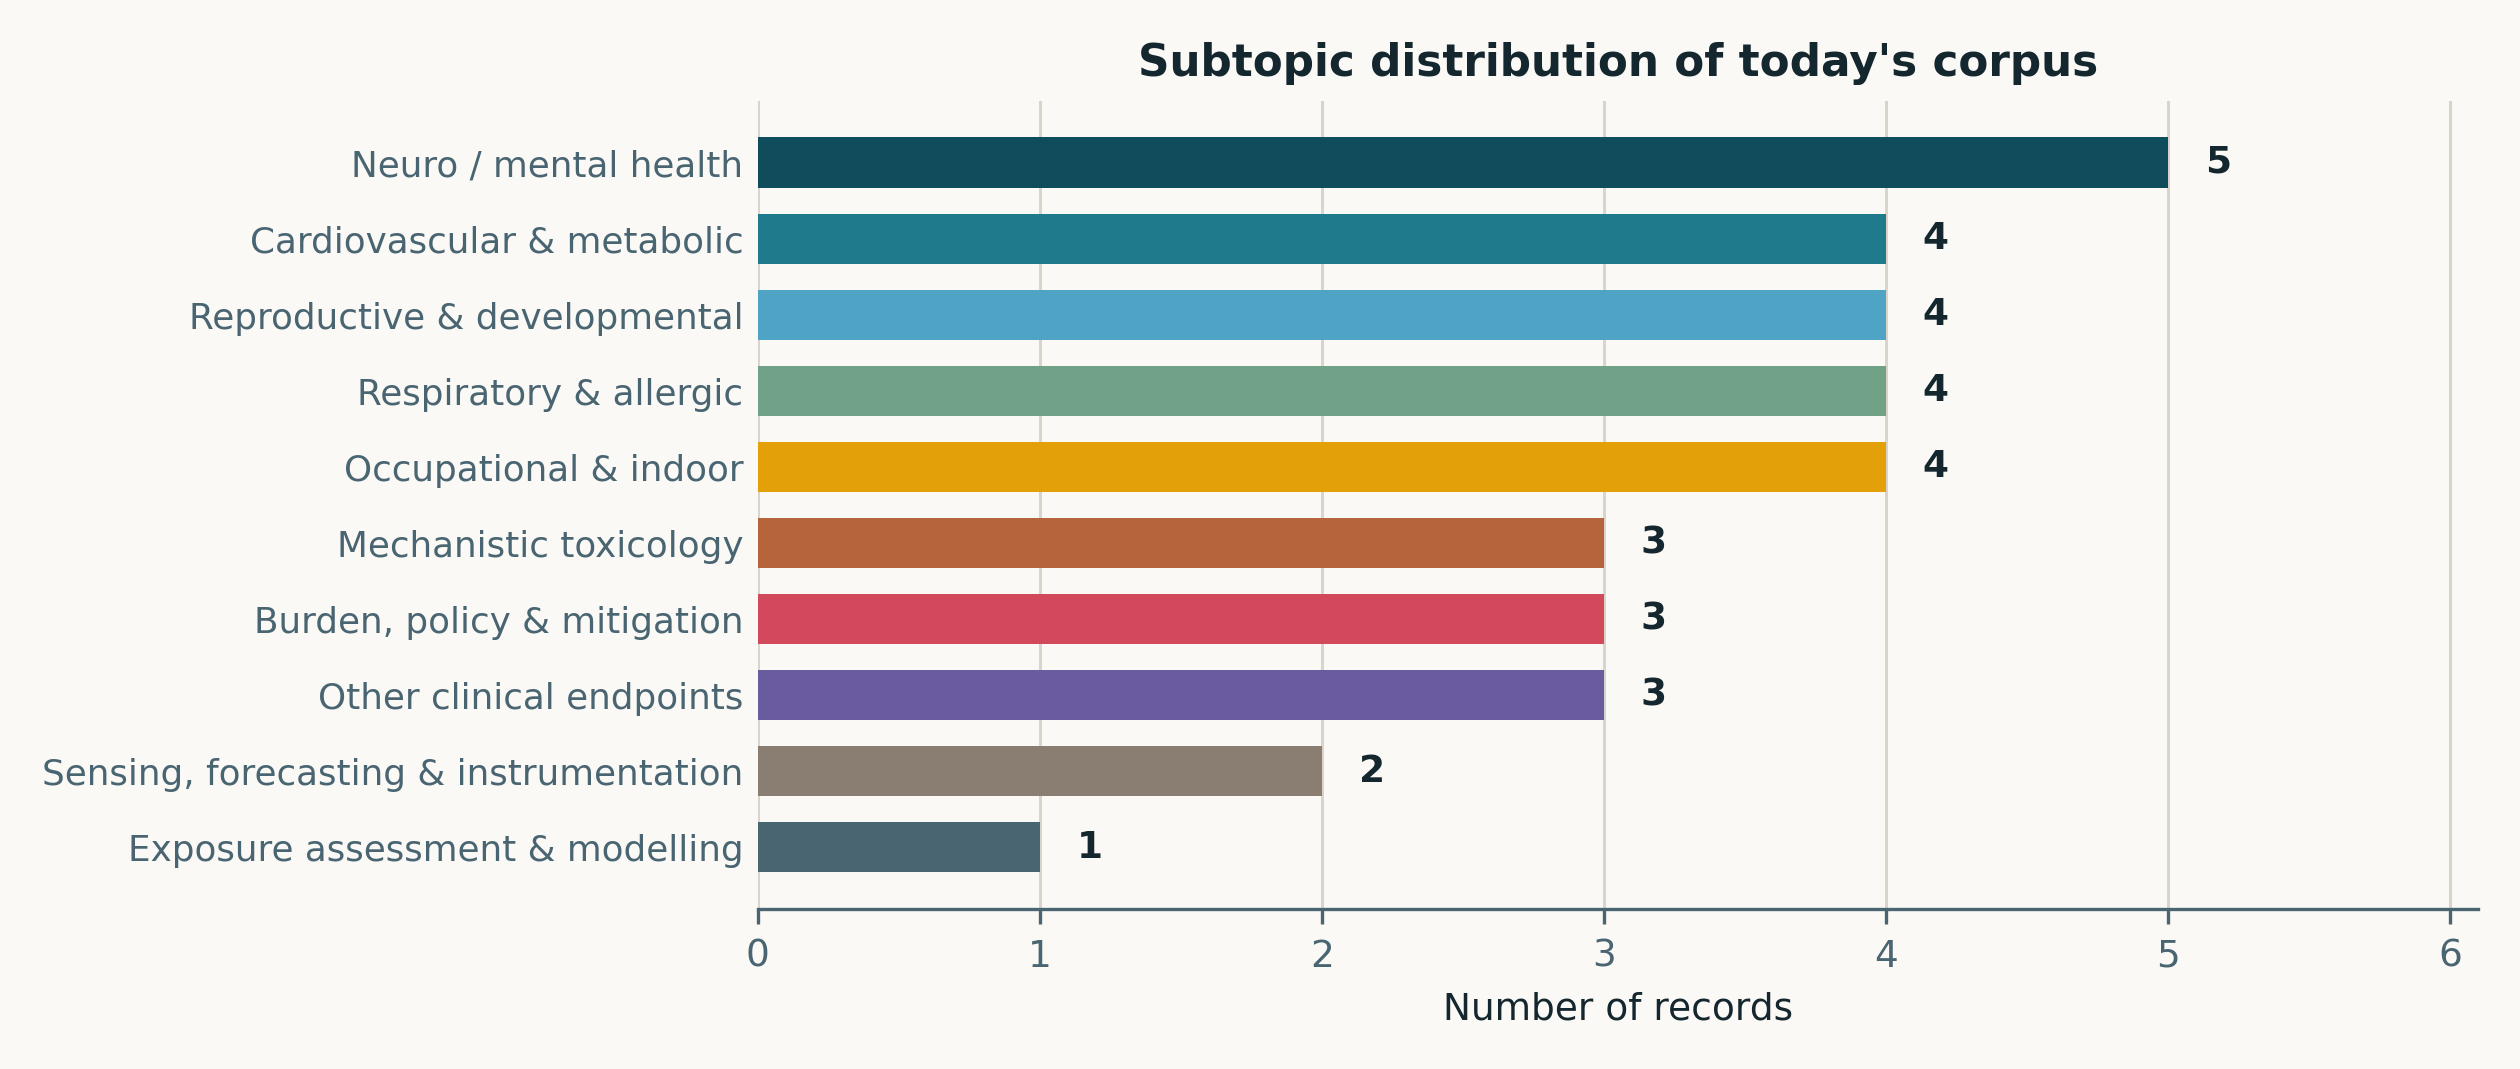
\includegraphics[width=\linewidth]{fig/f1_subtopics.png}
\figcap{Subtopic assignment of the 33 in-scope records. Assignment is single-label by
dominant contribution; several papers (e.g.\ prenatal-exposure cohorts) sit at the
boundary of \textit{Reproductive \& developmental} and \textit{Neuro}.
Neuro and mental-health work is the single largest cluster today (5), followed by four
clusters of four (cardiovascular/metabolic, reproductive/developmental,
respiratory/allergic, occupational/indoor).}

\vspace{2mm}
\noindent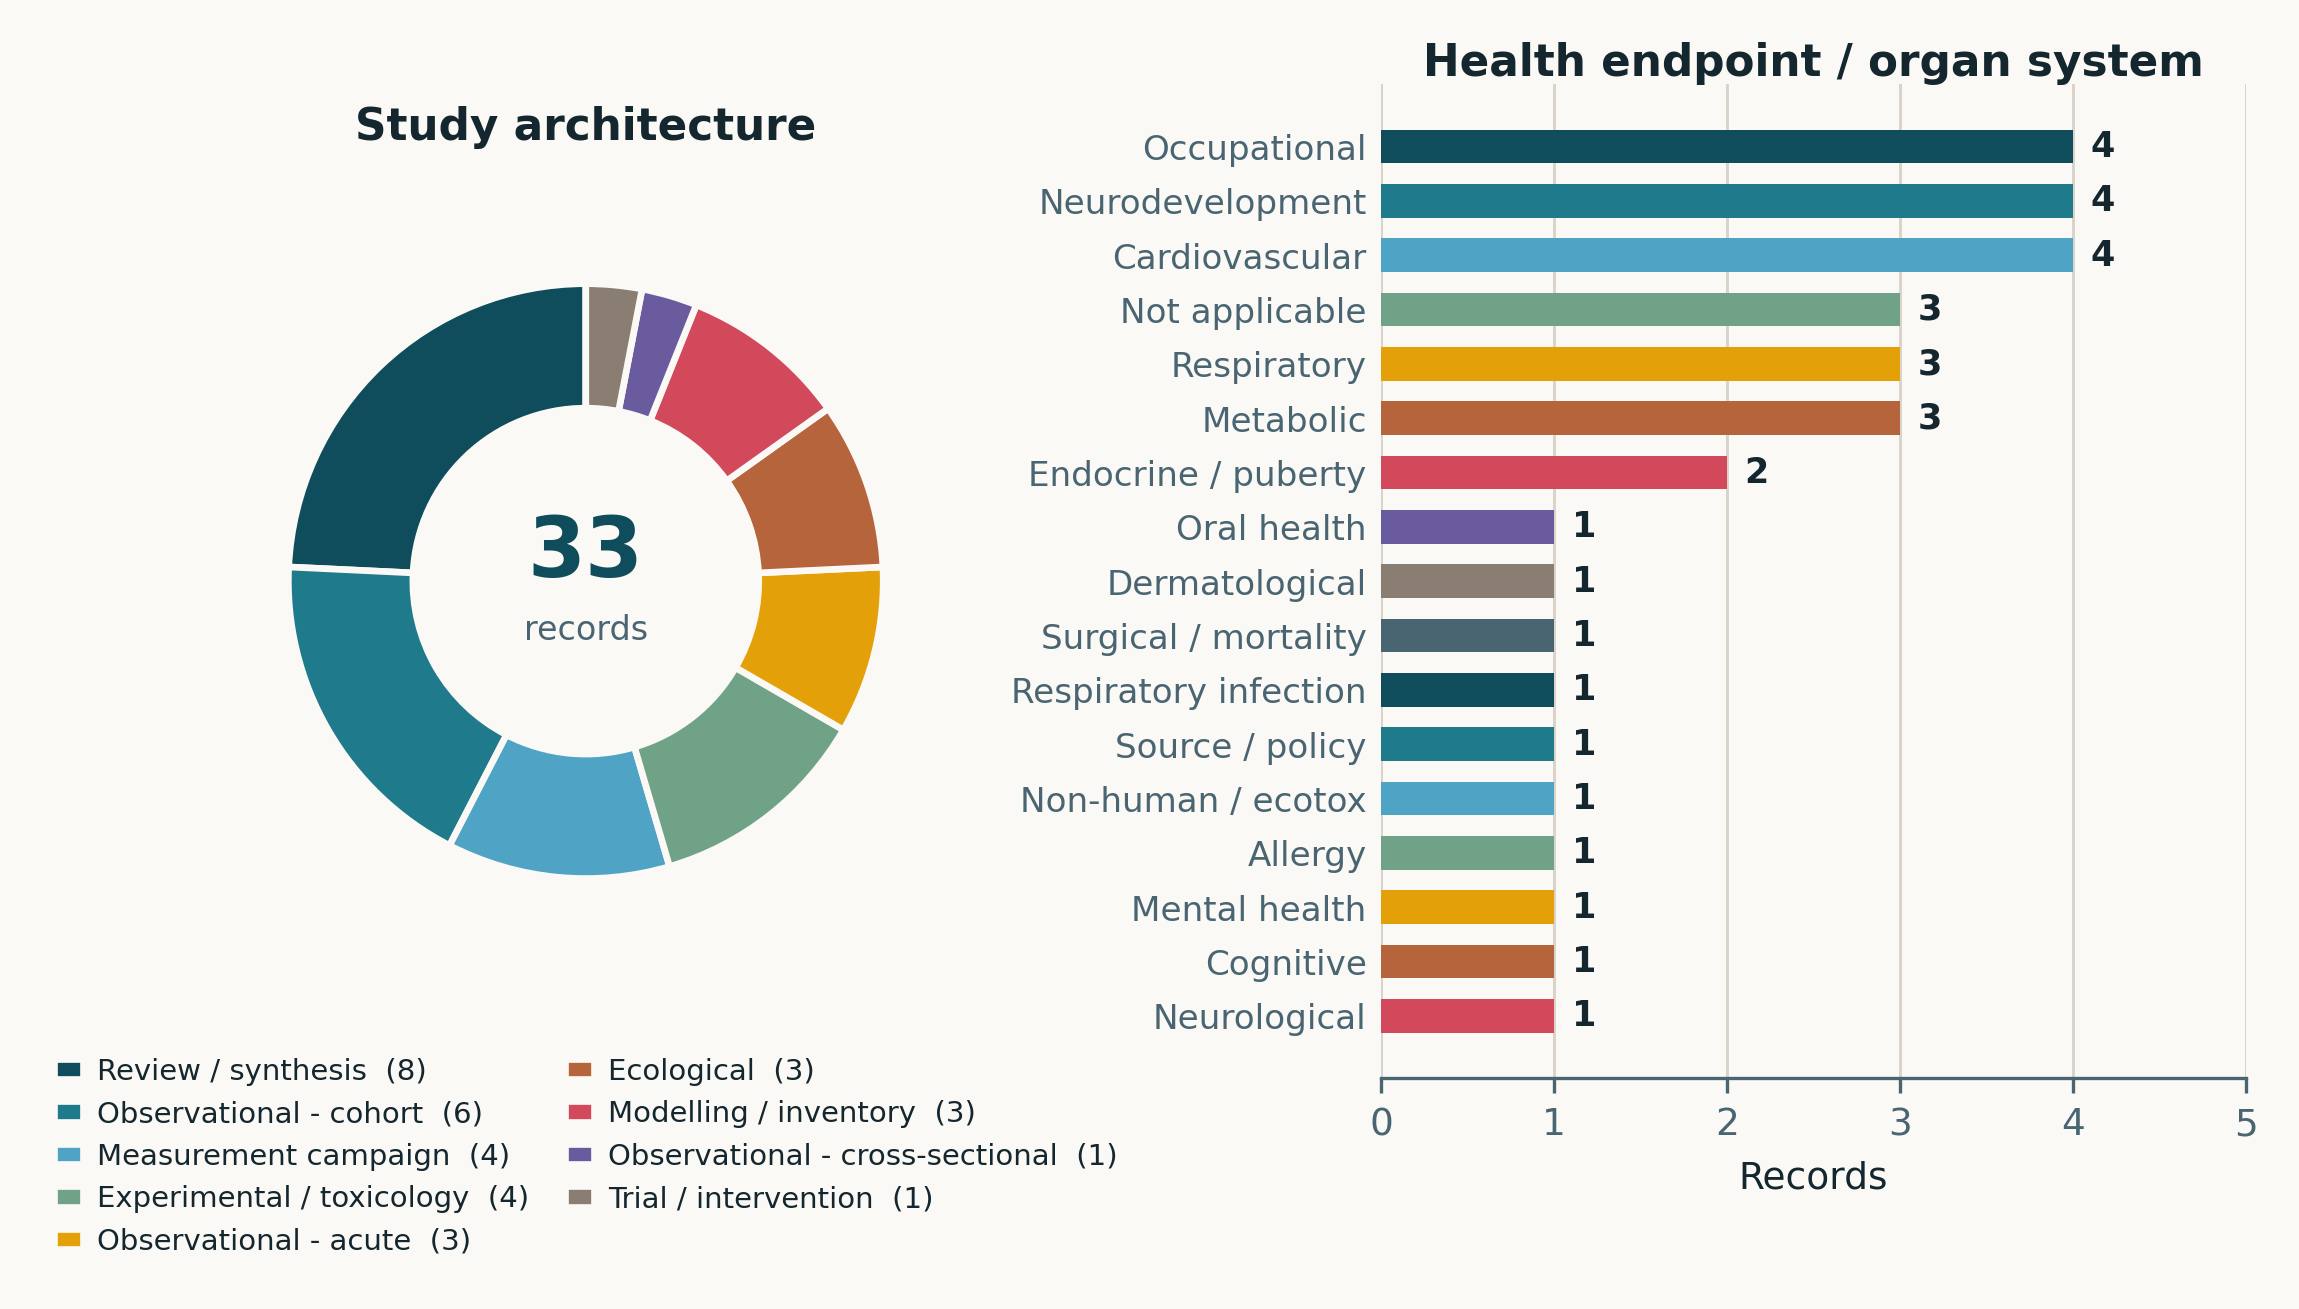
\includegraphics[width=\linewidth]{fig/f2_design_endpoint.png}
\figcap{Left --- study architecture. Reviews and syntheses account for 8/33 (24\%), an
unusually high share that reflects a cluster of mid-year review issues; primary
observational epidemiology (cohort, acute, cross-sectional) contributes 10.
Right --- health endpoint by organ system. Occupational, neurodevelopmental and
cardiovascular endpoints tie for the lead at four records each; five records carry no
human health endpoint at all (three pure monitoring/modelling, one emissions inventory,
one ecotoxicology).}

\vspace{2mm}
\noindent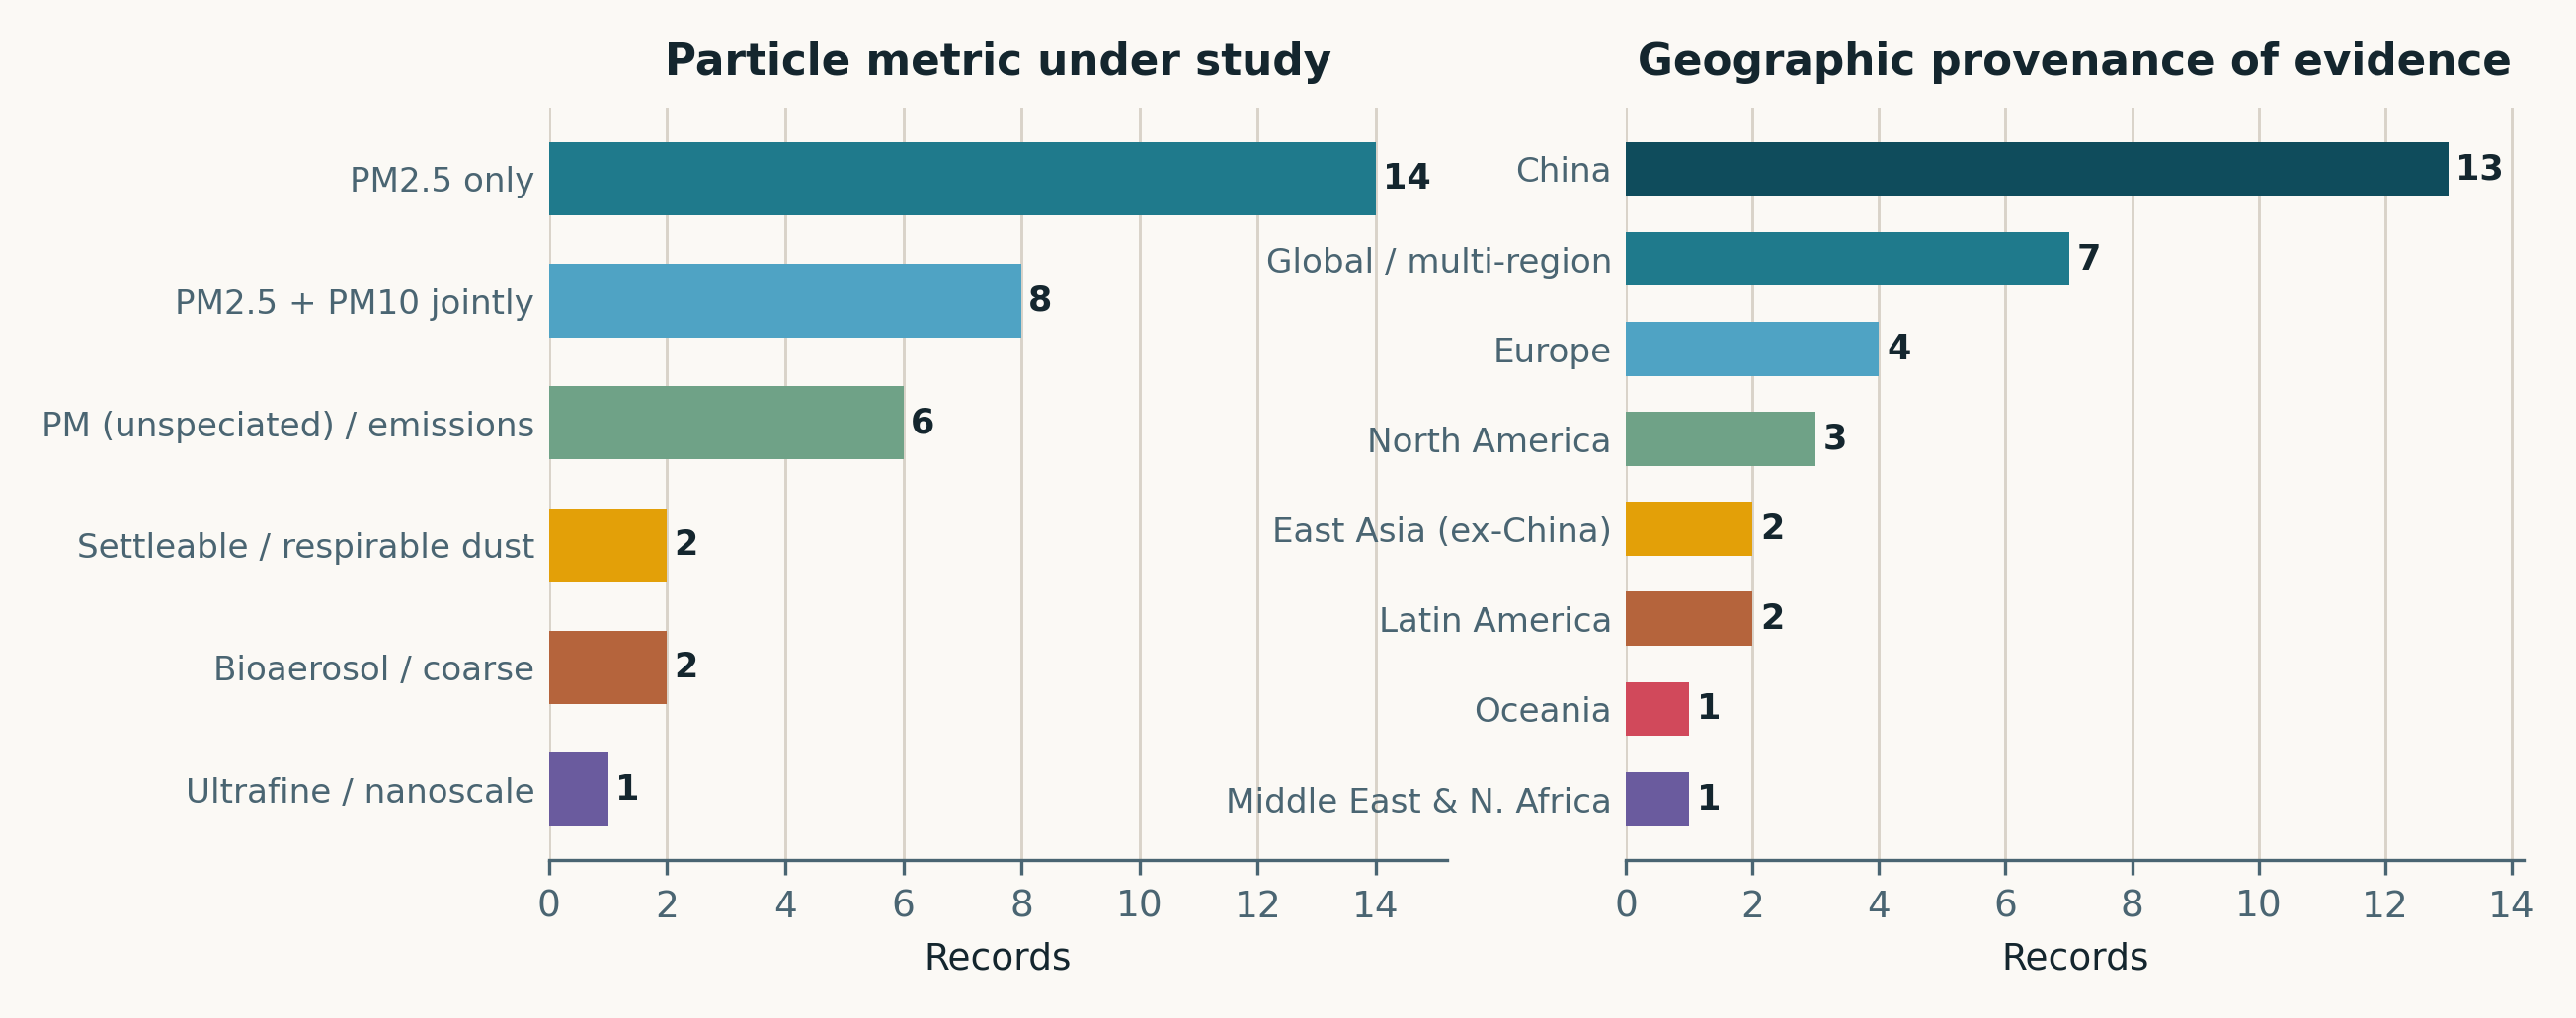
\includegraphics[width=\linewidth]{fig/f3_metric_geography.png}
\figcap{Left --- particle metric. PM$_{2.5}$ alone is the exposure in 14 records and
appears jointly with PM$_{10}$ in a further 8; ultrafine particles are the explicit
subject of only one record (aircraft cabin air), a persistent and notable gap given
the deposition physics. Right --- geographic provenance. China contributes 13 records
(39\%); no record today originates from South Asia or sub-Saharan Africa despite those
regions carrying the largest attributable burden.}

\vspace{2mm}
\noindent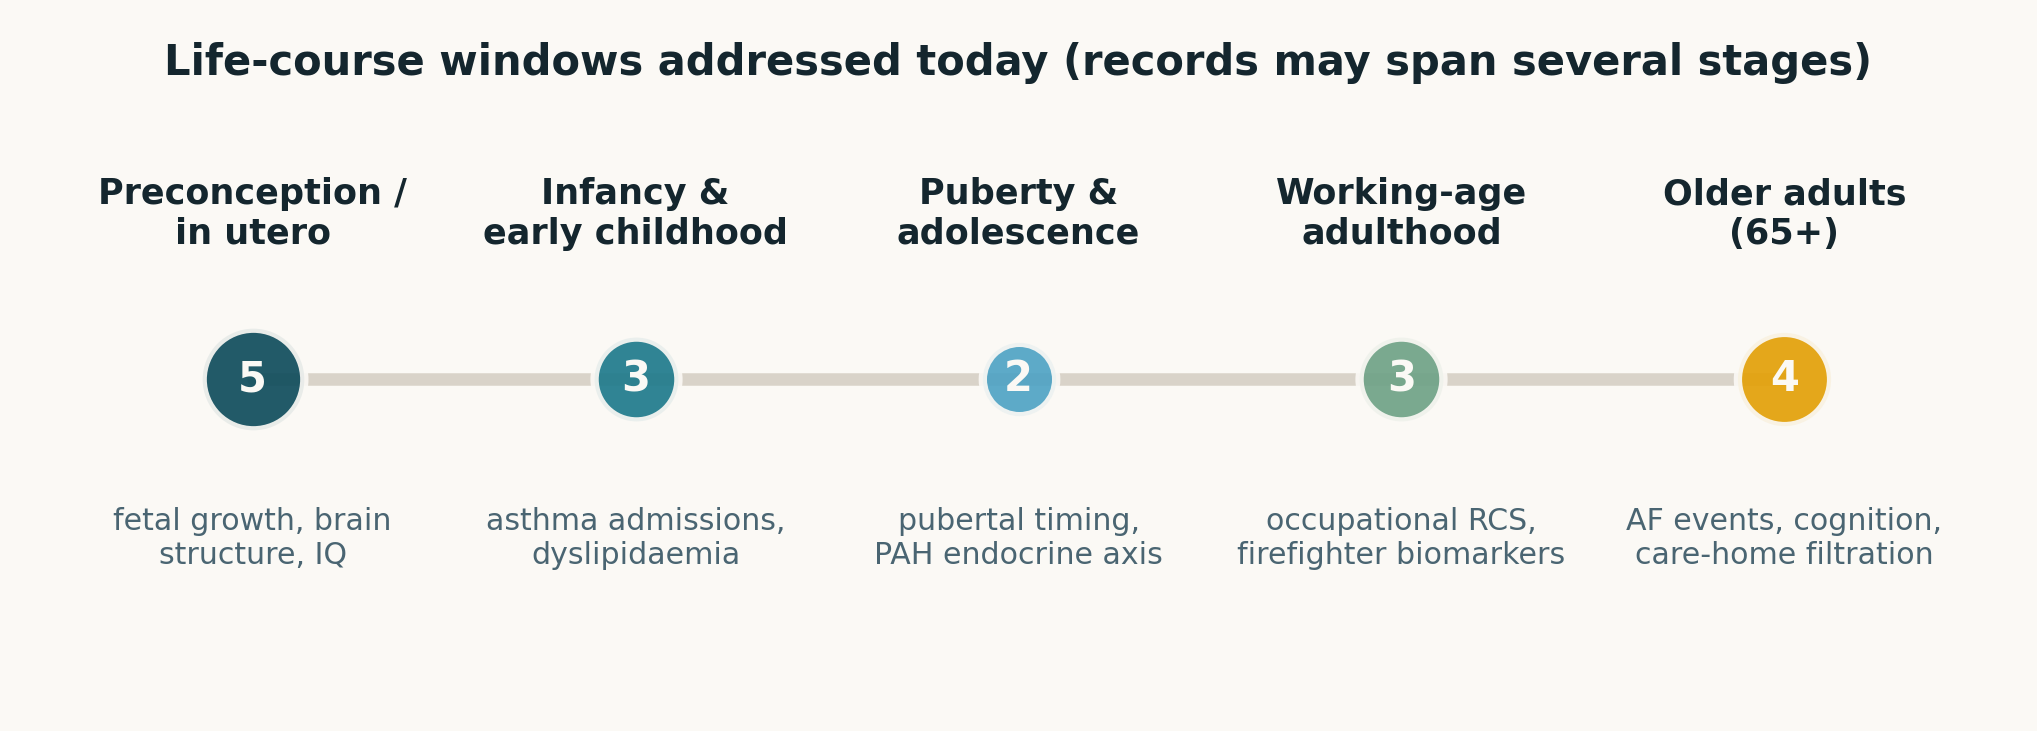
\includegraphics[width=\linewidth]{fig/f6_lifecourse.png}
\figcap{Life-course windows addressed. Counts are non-exclusive. The in-utero window
attracted the most attention today (5 records), consistent with the field's continuing
shift toward a developmental-origins framing.}

\vspace{2mm}
\noindent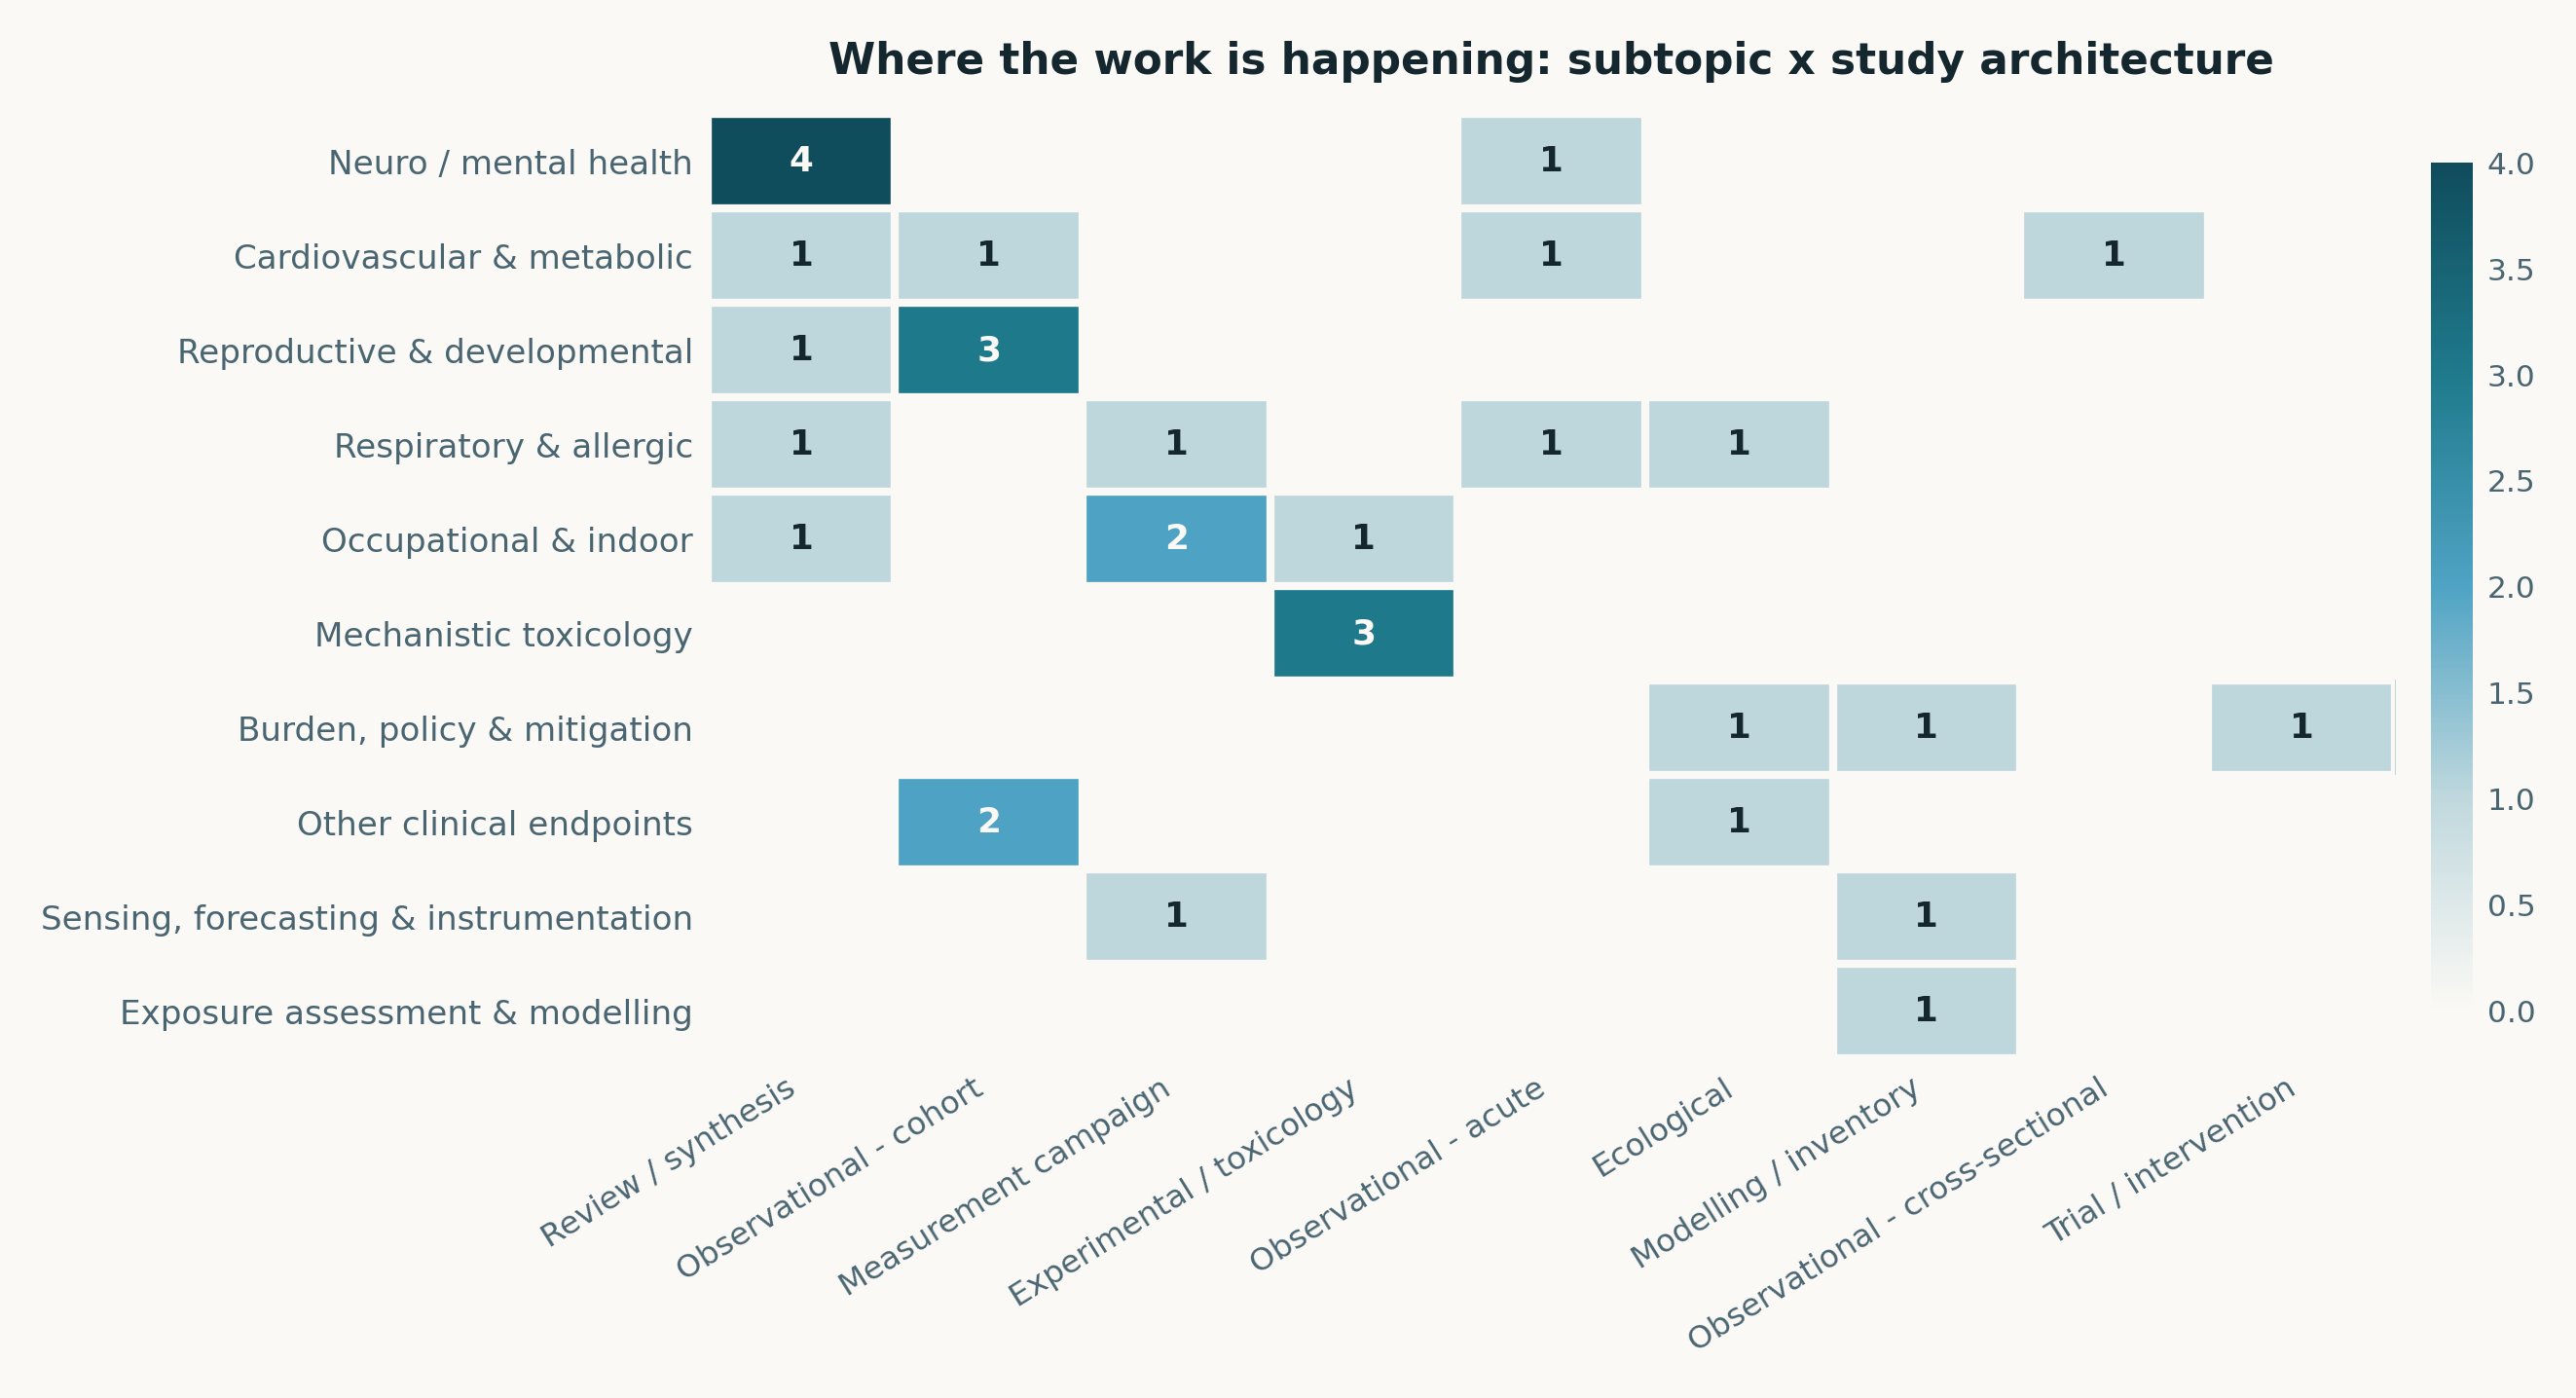
\includegraphics[width=\linewidth]{fig/f4_heatmap.png}
\figcap{Subtopic $\times$ study-architecture cross-tabulation. Two structural features
stand out: mechanistic toxicology is entirely experimental (3/3) with no bridge to human
biomarker work, and the \textit{Sensing / forecasting} and \textit{Exposure assessment}
rows contain no health-endpoint linkage at all --- instrumentation and epidemiology remain
methodologically siloed within today's harvest.}

\vspace{2mm}
\noindent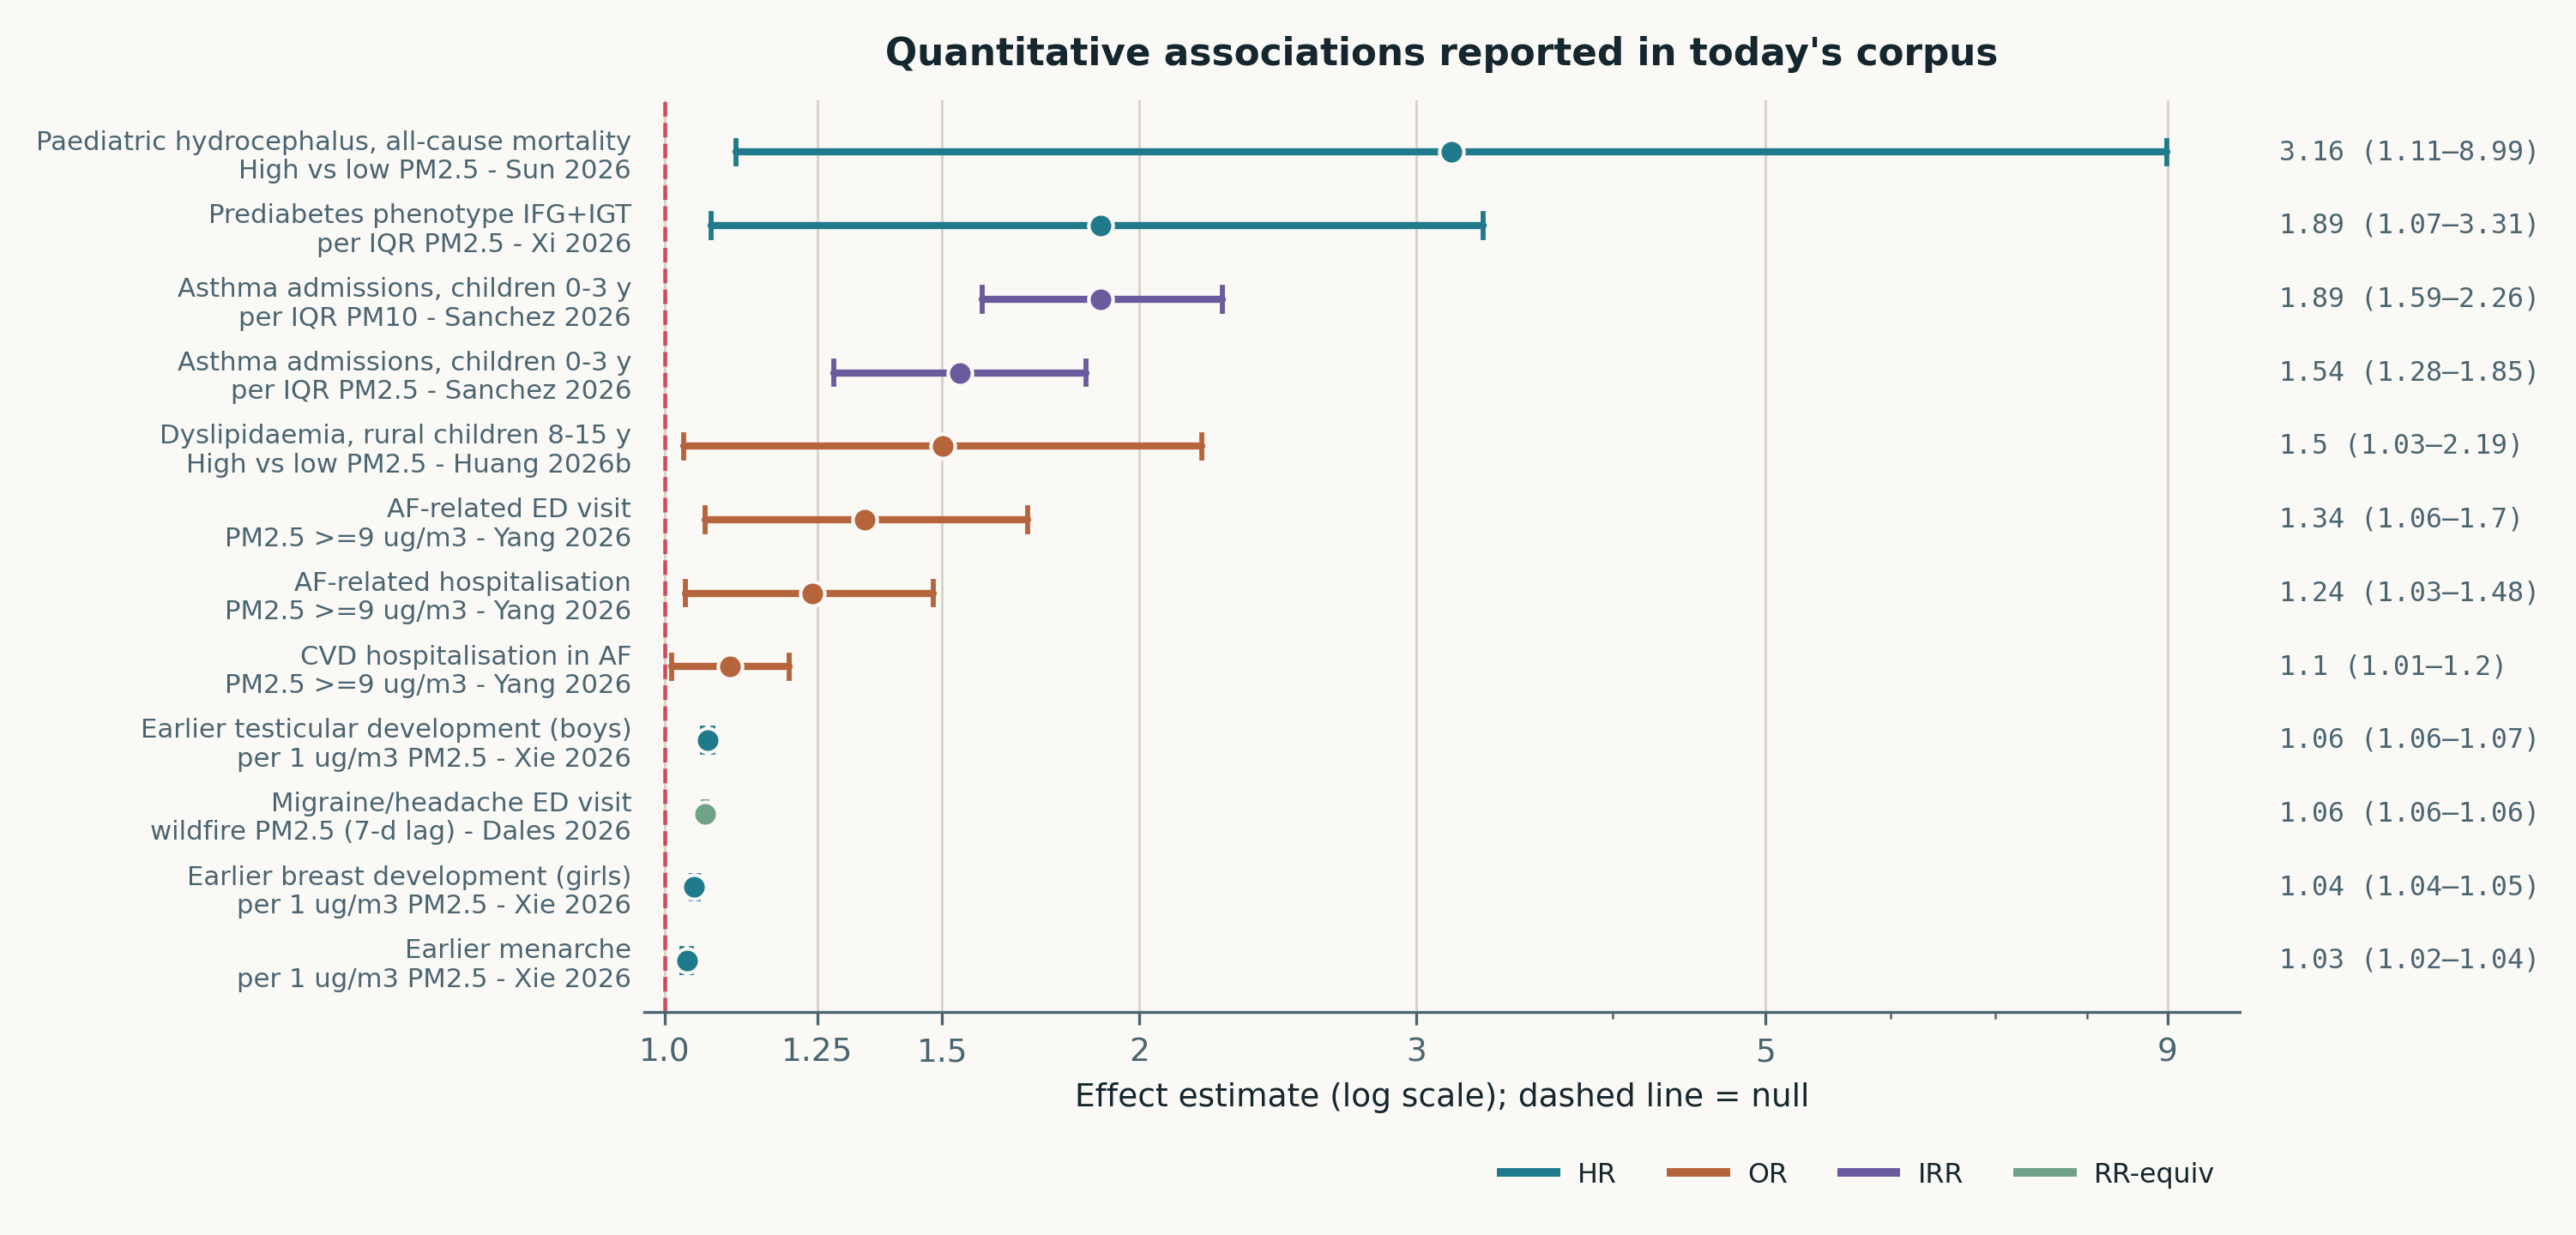
\includegraphics[width=\linewidth]{fig/f5_forest.png}
\figcap{All quantitative effect estimates reported across the corpus, on a common
logarithmic axis. \textbf{Exposure contrasts are heterogeneous and estimates are not
mutually comparable}: HRs from Xie et al.\ are per 1\,$\mu$g/m$^3$, Sanchez de Prada et al.\
report per-IQR IRRs, Yang et al.\ use a $\geq$9\,$\mu$g/m$^3$ threshold, and the Dales
et al.\ figure is a percentage-change converted to a risk-ratio equivalent. The plot is
intended to show \emph{precision and direction}, not relative magnitude. Note that the
tightest intervals (Xie, Dales) come from the largest samples and the widest (Sun,
paediatric hydrocephalus mortality) from an 881-patient registry.}

\clearpage

% ==================================================================== DIGEST
\section*{\sffamily\bfseries\color{Deep}Paper-level digest}
\vspace{-1.5mm}{\color{Amber}\rule{\linewidth}{1.1pt}}\vspace{1mm}

{\fontsize{7.4}{9}\selectfont\color{Slate}Ordered by cluster. Each entry gives the
methodological core and the finding that matters, not an abstract paraphrase.\par}

\band{Neuro, cognition \& mental health\hfill 5 records}{Deep}

\paperentry{Dales et al.\ 2026}
{Wildfire-sourced PM$_{2.5}$ and ED visits for migraine and other primary headache}
{JAMA Netw Open}
{Case-crossover over 997{,}701 ED visits, 2010--2023 Alberta/Ontario, using the Canadian
Optimized Statistical Smoke Exposure Model to separate wildfire-sourced from background
PM$_{2.5}$. \textbf{+6.07\% (5.75--6.39) per wildfire exposure}; background PM$_{2.5}$
null. Effect modification by material/social deprivation is large (3.61\% $\to$ 10.42\%
across quintiles). The methodological contribution --- explicit source attribution within a
case-crossover frame --- is more transferable than the headache endpoint itself.}
{10.1001/jamanetworkopen.2026.25015}

\paperentry{Glover et al.\ 2026}
{Umbrella meta-review of urban environmental exposures and cognitive health}
{Age Ageing}
{54 systematic reviews, 66 meta-analysed outcomes, 270 exposure--outcome associations,
graded by sample size, effect strength and bias. PM$_{2.5}$ is the strongest-graded
exposure (10/11 significant outcomes, ``highly probable'' detrimental), ahead of
NO$_2$/NO$_x$ (5/10). Social relationships were probably protective; green/blue space
associated with lower dementia risk (3/6). Useful as a citation anchor for exposure
hierarchy claims.}
{10.1093/ageing/afag215}

\paperentry{Ma \& Yau 2026}
{PM$_{2.5}$-induced neurotoxicity and depression: exposure risks and mechanisms}
{iScience}
{Narrative integration of epidemiological, animal and mechanistic evidence.
Component-focused: metals, black carbon and organic compounds are implicated via
oxidative stress, neuroinflammation, blood--brain barrier disruption, HPA-axis
dysregulation and kynurenine-pathway alteration. Explicitly calls for
component-resolved exposure assessment --- relevant if your instrumentation work can
deliver speciated output.}
{10.1016/j.isci.2026.116617}

\paperentry{Goossens et al.\ 2026}
{In utero air pollution exposure and pre-/postnatal brain development}
{Neurosci Appl}
{Imaging-focused review (fetal ultrasound + childhood/adolescent MRI) stratified by
pollutant. Prenatal ultrasound studies in high-exposure regions show reduced biparietal
diameter and head circumference; childhood MRI in low-exposure regions shows no global
volume effect but regional cortical, subcortical grey and white matter differences.
The exposure-contrast dependence of the discrepancy is the point worth carrying forward.}
{10.1016/j.nsa.2026.107019}

\paperentry{Pan et al.\ 2026}
{Maternal PM exposure and offspring neurodevelopment: effects and mechanisms}
{Zhonghua Yu Fang Yi Xue Za Zhi}
{Chinese-language review covering placental barrier disruption and particle
translocation, oxidative stress, epigenetic alteration, endocrine dysfunction and gut
microbiota imbalance. Largely confirmatory of the above; included for completeness of
the mechanistic map.}
{10.3760/cma.j.cn112150-20250804-00752}

\band{Cardiovascular \& metabolic\hfill 4 records}{Teal}

\paperentry{Yang et al.\ 2026}
{Short-term PM$_{2.5}$ and hospitalisation/ED use in atrial fibrillation}
{J Am Heart Assoc}
{2021 Medicare data, 26{,}158 western-US patients with established AF; ZIP-code daily
PM$_{2.5}$ from a 1\,km geospatial model, threshold $\geq$9\,$\mu$g/m$^3$, lags 0/1/3\,d.
\textbf{OR 1.10 (1.01--1.20) for CVD hospitalisation; 1.24 (1.03--1.48) for AF
hospitalisation; 1.34 (1.06--1.70) for AF ED visits.} No significant PM$\times$extreme-heat
interaction --- a negative finding worth noting given how often synergy is assumed.}
{10.1161/JAHA.125.046917}

\paperentry{Xi et al.\ 2026}
{Air pollution, built environment and temperature vs.\ prediabetes phenotypes (KORA)}
{Diabetologia}
{KORA cohort, Southern Germany 2006--2022, 1{,}618 participants, complementary log-log
models plus quantile g-computation for mixtures. Per-IQR PM$_{2.5}$ gave
\textbf{HR 1.89 (1.07--3.31) for combined IFG+IGT}; lower NDVI HR 1.59 (1.03--2.46).
Crucially, associations were with \emph{incidence and non-remission} of impaired glucose
tolerance rather than progression to type 2 diabetes --- a phenotype-resolution result
that most air-pollution/diabetes studies cannot deliver.}
{10.1007/s00125-026-06814-2}

\paperentry{Huang et al.\ 2026}
{PM$_{2.5}$ and dyslipidaemia in rural Chinese children; dietary effect modification}
{Zhonghua Liu Xing Bing Xue Za Zhi}
{10{,}788 children aged 8--15 across 103 surveillance counties; 3-year mean PM$_{2.5}$
30.36$\pm$10.62\,$\mu$g/m$^3$; dyslipidaemia prevalence 21.84\%. \textbf{OR 1.501
(1.028--2.192)}, with no significant association among children with greater vegetable
intake diversity. Effect-modification-by-diet claims of this type are fragile to
residual confounding, but the sample size is substantial.}
{10.3760/cma.j.cn112338-20251120-00843}

\paperentry{Ka\'zmierska et al.\ 2026}
{Air pollution and cardiovascular disease: review of current data}
{Przegl Epidemiol}
{Standard mechanistic review (oxidative stress, inflammation, endothelial dysfunction,
autonomic imbalance) anchored to the 2021 WHO 5\,$\mu$g/m$^3$ annual guideline. Adds
little new; useful only as an introductory citation.}
{10.32394/pe/218966}

\band{Reproductive \& developmental\hfill 4 records}{Sky}

\paperentry{Xie et al.\ 2026}
{Long-term PM$_{2.5}$ and timing of pubertal development in boys and girls}
{Environ Res}
{Chongqing Child Health Cohort 2014--2024, 3{,}833 children, time-varying cumulative
average residential PM$_{2.5}$ from the prenatal period, Cox models across nine
milestones. \textbf{Boys: testicular HR 1.065 (1.056--1.073), penile 1.063
(1.055--1.071). Girls: breast 1.044 (1.039--1.050), menarche 1.033 (1.025--1.040),}
all per 1\,$\mu$g/m$^3$. Associations were stronger in overweight/obese girls and in
areas with higher long-term temperature and lower humidity --- i.e.\ meteorological
effect modification, not just confounding. The male-inclusive design is the field's
main gap being closed here.}
{10.1016/j.envres.2026.125313}

\paperentry{Peterson 2026}
{Ambient air pollution, PAHs and pubertal development: critical review}
{Curr Environ Health Rep}
{Component-level synthesis. Organic matter and sulfate fractions of PM$_{2.5}$ are
associated with earlier menarche and precocious puberty; OM is enriched in
combustion-derived PAHs. Notably, high \emph{chronic} exposure in heavily polluted
settings has also been associated with \emph{delayed} menarche --- a non-monotonic pattern
that any dose--response modelling should accommodate. Proposed mechanism: disruption of
hypothalamic kisspeptin--GnRH signalling.}
{10.1007/s40572-026-00552-8}

\paperentry{Huang et al.\ 2026}
{Joint prenatal bisphenol + air-pollutant mixture exposure and preschool IQ}
{Ecotoxicol Environ Saf}
{Guangxi Zhuang Birth Cohort, 231 mother--child pairs, WISC indices, analysed by
generalized linear models, restricted cubic splines, PCA, quantile g-computation and
BKMR. Prenatal PM$_{2.5}$ and PM$_{10}$ associated with lower verbal comprehension and
full-scale IQ; effects stronger in boys; BKMR shows an inverted-U for fluid reasoning
against the 10-pollutant mixture. Small $n$ --- treat the mixture results as
hypothesis-generating.}
{10.1016/j.ecoenv.2026.120566}

\paperentry{Chen et al.\ 2026}
{Prenatal air pollution, fetal growth trajectories and child neurodevelopment}
{J Environ Sci (China)}
{Time-series $k$-means clustering to derive fetal growth trajectory phenotypes, then
mediation analysis. Sensitive windows identified at 0--20 and 27--41 weeks; higher
exposure raised odds of high-risk trajectories by 9--32\%, and first-trimester
crown--rump length plus mid-pregnancy estimated fetal weight mediated effects on the
2-year psychomotor development index. The trajectory-clustering approach is the
methodologically interesting part.}
{10.1016/j.jes.2025.10.043}

\clearpage

\band{Respiratory \& allergic\hfill 4 records}{Sage}

\paperentry{S\'anchez de Prada et al.\ 2026}
{Ambient PM and asthma-coded admissions in children aged 0--3, Spain}
{Epidemiologia}
{Nationwide municipality-year ecological panel, 2020--2022, 20{,}746 municipality-years,
3{,}231 admissions --- but 93.7\% of municipality-years are zero, which is the dominant
statistical feature. Poisson IRRs per IQR: \textbf{PM$_{2.5}$ 1.54 (1.28--1.85),
PM$_{10}$ 1.89 (1.59--2.26)}; attenuated but persistent under negative-binomial and
province fixed effects. Multipollutant models were collinear and unstable. Ecological
design --- do not read as individual-level risk.}
{10.3390/epidemiologia7040097}

\paperentry{Yang et al.\ 2026}
{Allergenic vs.\ toxic risk of airborne seed hairs compared with ambient PM$_{2.5}$}
{J Hazard Mater}
{Simultaneous urban/suburban sampling of poplar-willow seed hairs and PM$_{2.5}$ in
Hohhot, May 2025, with sIgE-based allergenic quantification and FVOC/heavy-metal
toxicity. Seed hairs carry 13.1$\pm$12.1$\times$ the pollen and 92.9$\pm$55.2$\times$ the
bacterial load per unit mass, giving sIgE levels 14.9$\times$ and 124$\times$ higher than
concurrent PM$_{2.5}$; conversely PM$_{2.5}$ FVOC toxicity exceeds seed hairs by
$\sim$4$\times$10$^4$. A clean demonstration that mass-based monitoring misallocates
seasonal allergenic risk entirely.}
{10.1016/j.jhazmat.2026.143076}

\paperentry{Liao et al.\ 2026}
{Short-term air pollution, respiratory symptoms and lung function in asthma}
{Med Gas Res}
{Small panel study (32 patients, 266 visits, Beijing 2015--2016) with mixed-effects
models. Per-IQR PM$_{2.5}$ (74.5\,$\mu$g/m$^3$, 6-day) reduced Asthma Control Test
scores 3.6\%; PM$_{10}$ 7-day moving average reduced FEV$_1$\% predicted by 3.6\% and
FEF$_{25}$\% by 6.0\%. Exposure levels are far above current WHO guidance --- limits
extrapolation to low-exposure settings.}
{10.4103/mgr.MEDGASRES-D-25-00164}

\paperentry{Bayar Muluk 2026}
{Climate change and otolaryngology: airway disease and surgical emission reduction}
{Int J Biometeorol}
{Dual-domain narrative review. The relevant claim is a proposed \emph{synergy} between
elevated CO$_2$ and PM$_{2.5}$ increasing pollen allergenicity and mucosal penetration.
The second half (operating-room carbon footprint) is outside this watch's scope.}
{10.1007/s00484-026-03289-z}

\band{Mechanistic toxicology\hfill 3 records}{Violet}

\paperentry{Ding et al.\ 2026}
{PM$_{2.5}$ promotes vascular calcification via miR-27b-5p/HES1 signalling}
{J Environ Sci (China)}
{Mouse aortic smooth-muscle cells, hiPSC-derived 3D blood-vessel organoids, and a murine
model. Proposed axis: PM$_{2.5}$ suppresses miR-27b-5p transcription in an XBP1-dependent
manner $\to$ HES1--Runx2 interaction $\to$ osteogenic transformation of VSMCs.
miR-27b-5p mimics rescued the organoid phenotype. The organoid arm is the credible
translational bridge; dose and duration dependence shown in vivo.}
{10.1016/j.jes.2025.12.074}

\paperentry{Wu et al.\ 2026}
{Macrophage NLRP3 inflammasome in real-ambient PM-induced hepatic glucose dysregulation}
{J Environ Sci (China)}
{Individually-ventilated-cage real-ambient exposure system, 15 weeks, plus transwell
macrophage--hepatocyte co-culture and \textit{Nlrp3} knockdown. Lysosomal damage and
cathepsin B release $\to$ NLRP3 activation $\to$ IL-1$\beta$ $\to$ suppressed hepatocyte
insulin signalling. Both NLRP3 inhibition and IL-1$\beta$ blockade rescued.
Real-ambient exposure (rather than instillation) makes the dosimetry considerably more
defensible than most of this literature.}
{10.1016/j.jes.2025.11.018}

\paperentry{Maraschi et al.\ 2026}
{Osmoregulatory disruption from settleable atmospheric PM in estuarine fish}
{J Comp Physiol B}
{96\,h exposure of \textit{Centropomus parallelus} to 1\,g\,L$^{-1}$ settleable APM.
Al, Fe, V and Cr accumulated in gill and kidney; branchial Na$^+$/K$^+$-ATPase activity
and NKA$^+$ ionocyte density rose while renal ATPase activity fell. Ecotoxicological
rather than human-health relevant, but a useful reminder that deposition, not
inhalation, is the dominant PM pathway in aquatic receptors.}
{10.1007/s00360-026-01698-5}

\band{Occupational \& indoor exposure\hfill 4 records}{Clay}

\paperentry{Cole \& Driscoll 2026}
{Determinants of respirable crystalline silica exposure in Australian tunnelling}
{Ann Work Expo Health}
{3{,}288 personal exposure measurements across 12 tunnel projects (2016--2024), obtained
via freedom-of-information requests --- the largest such dataset in Australian tunnelling.
Linear mixed models explained 53--68\% of variance. Underground workers had
\textbf{2.3$\times$ the exposure of above-ground workers} (GM 0.026 vs.\ 0.012\,mg/m$^3$);
each 1\% increase in silica fraction of respirable dust raised RCS exposure 5\%;
exposures fell after the July 2020 standard reduction (GM 0.023 $\to$ 0.013\,mg/m$^3$).
A model for what transparent exposure-data access enables.}
{10.1093/annweh/wxag055}

\paperentry{Ding et al.\ 2026}
{Stage-resolved hair Zn-isotope dynamics as a firefighting exposure tracer}
{J Hazard Mater}
{53 hair samples from 15 Beijing firefighters across five stage-defined periods.
$\delta^{66}$Zn ranged $-$0.79 to $-$0.13\permil, with non-linear
incident--recovery trajectory: heavy-isotope enrichment after repeated missions,
partial return toward baseline in late recovery. Linear mixed effects with stage-dependent
Ni/Pb/Co associations; ICC 0.82 (i.e.\ dominated by between-subject variability).
A genuinely novel time-integrated biomarker concept for combustion-derived PM.}
{10.1016/j.jhazmat.2026.143081}

\paperentry{Tsuchiya et al.\ 2026}
{Seasonal and indoor--outdoor characteristics of fluorescent aerosol particles in offices}
{Biosensors}
{Real-time bioaerosol sensor across 10 office spaces in four Japanese regions, summer and
winter. Indoor FAP generally $<$100\,particles\,L$^{-1}$, peaking at 195\,p/L in winter;
several buildings higher in winter, attributed to RH$<$40\% promoting resuspension.
Size-resolved FAP fraction rises sharply with diameter (40--74\% at 2--5\,$\mu$m;
96--100\% $>$5\,$\mu$m). Directly relevant to anyone deploying optical/fluorescence
sensors --- the coarse-mode dominance constrains what a fluorescence channel can be
interpreted to mean.}
{10.3390/bios16070380}

\paperentry{Ramsden 2026}
{Xenobiotic hazards in aircraft cabin air}
{J Xenobiot}
{Review of bleed-air contamination in the $\sim$95\% of airliners drawing cabin air from
turbine compressors: engine-oil traces, tricresyl phosphate, and ultrafine particles
abraded from turbine blades. Argues no safe lower TCP limit given inter-individual
sensitivity, and presents a life-quality-index affordability calculation.
The only ultrafine-focused record in today's corpus.}
{10.3390/jox16040119}

\clearpage

\band{Sensing, forecasting \& exposure modelling\hfill 3 records}{Amber}

\paperentry{Shi et al.\ 2026}
{Adaptive Spatiotemporal Graph Transformer for multi-site multi-step PM$_{2.5}$ forecasting}
{J Environ Manage}
{AST-GT with five components: adaptive non-stationary normalisation for time-varying
distribution drift; Transformer temporal encoding; multi-source context fusion
(geography, meteorology, co-pollutants); graph-based dual-scale spatial attention; and a
temporal--spatial cooperative attention block. Validated on Beijing and India multi-site
datasets. The non-stationarity handling and the explicit treatment of \emph{uneven site
distribution} are the parts worth reading if you work with sparse monitoring networks.}
{10.1016/j.jenvman.2026.130515}

\paperentry{Sol\'orzano-Araque et al.\ 2026}
{Multiscale exposure modelling with LOTOS-EUROS, mobility surveys and particle toxicity}
{GeoHealth}
{Medell\'in / Aburr\'a Valley, 2019. LOTOS-EUROS CTM driven by WRF at
1\,km$\times$1\,km; mobility from an origin--destination survey of $>$180{,}000 trips across
240 traffic analysis zones; morpho-chemical characterisation of metals and carbonaceous
fractions; and a weighted exposure model combining exposure time, concentration and
cytogenotoxic indicators. Cluster analysis identified central and southern zones and
highway corridors --- $\sim$60\% of the metropolitan population --- exceeding
40\,$\mu$g/m$^3$ at peak hours. The toxicity-weighting step is the transferable idea.}
{10.1029/2025GH001621}

\paperentry{Chen et al.\ 2026}
{Nested suction instrument to reduce intraoperative surgical-smoke PM$_{2.5}$}
{Front Med Technol}
{Bench study on porcine dorsal tissue with electrosurgical cutting, PM$_{2.5}$ monitored
by laser dust counters. Three orifice diameters tested (1.5/2.0/2.5\,mm) with local smoke
evacuation; reduction rates 24.2\%, 66.9\% and 43.0\% respectively --- the 2.0\,mm
``all-in-one'' design (simultaneous smoke and blood suction) was optimal. Small,
single-setting, but a clean engineering-control result.}
{10.3389/fmedt.2026.1796828}

\band{Burden, policy \& mitigation\hfill 3 records}{Coral}

\paperentry{Karamzad et al.\ 2026}
{Ischaemic heart disease burden in MENA, 1990--2021 (GBD 2021)}
{Health Sci Rep}
{21 countries. 2021 age-standardised IHD prevalence 6{,}404.8/100{,}000, mortality
202.8, DALY rate 4{,}023.2. \textbf{Ambient PM pollution accounts for 28.2\% of IHD
DALYs}, third after systolic blood pressure (49.6\%) and LDL cholesterol (39.6\%).
Age-standardised rates declined 1990--2021 but burden remains high and inversely
non-linearly related to SDI.}
{10.1002/hsr2.72886}

\paperentry{Shan et al.\ 2026}
{Policy-driven emission reductions and post-pandemic rebound in China}
{J Environ Sci (China)}
{High-resolution integrative inventories for 2018, 2020 and 2023 covering CO$_2$ and nine
pollutants. In 2020 vs.\ 2018, SO$_2$ ($-$18.1\%), VOCs ($-$32.6\%) and CO ($-$8.8\%) fell
while CO$_2$ (+11.6\%), NO$_x$ (+16.8\%) and PM (+21.9\%) rose on expanded power
generation and metal production. 2023 saw 3.2--15.1\% rebound across pollutants.
The Fenwei Plain shows persistent PM growth. Useful for anyone building
policy-counterfactual exposure scenarios.}
{10.1016/j.jes.2026.01.009}

\paperentry{Rees et al.\ 2026}
{AFRI-c HEPA filtration in care homes: mixed-methods process evaluation}
{PLoS One}
{Process evaluation of a cluster RCT across 22 care homes (25 staff, 20 resident and 12
relative interviews; 1{,}158 resident questionnaires), using normalisation process
theory. Self-reported fidelity was high with low contamination --- \textbf{the trial's null
infection result is therefore unlikely to be an adherence artefact}. HEPA units did not
change infection-control practice or environmental satisfaction; some residents disliked
the draught. An important negative-result anchor for indoor filtration claims.}
{10.1371/journal.pone.0347989}

\band{Other clinical endpoints\hfill 3 records}{Slate}

\paperentry{Sun et al.\ 2026}
{Environmental exposure and area deprivation vs.\ paediatric hydrocephalus outcomes}
{J Neurosurg Pediatr}
{881 patients, 2008--2023 single-institution registry, geocoded to Area Deprivation Index
and CDC/ATSDR environmental measures plus satellite-derived ground-level PM$_{2.5}$.
Multivariable Cox with cluster-robust SEs: high ozone HR 1.38 (1.05--1.82) and high ADI
HR 1.46 (1.15--1.86) for shunt failure; high coal exposure HR 1.92 (1.28--2.88) for shunt
infection; \textbf{high PM$_{2.5}$ HR 3.16 (1.11--8.99) for all-cause mortality}.
The mortality CI is very wide --- treat as signal, not estimate.}
{10.3171/2026.3.PEDS2615}

\paperentry{Park et al.\ 2026}
{Long-term particulate matter exposure and risk of androgenetic alopecia}
{JAAD Int}
{Nationwide Korean cohort research letter linking long-term PM$_{2.5}$/PM$_{10}$ to
androgenetic alopecia incidence, with hair-follicle inflammation and oxidative stress as
the proposed mechanism. Abstract not indexed; full text required for effect sizes.}
{10.1016/j.jdin.2026.06.008}

\paperentry{Lupita et al.\ 2026}
{PM$_{2.5}$, preventive-care capacity and oral disease burden across the EU}
{Dent J}
{Ecological panel across 27 EU member states, 2020--2023, GBD outcomes vs.\ national mean
PM$_{2.5}$ with unmet dental care need as an effect modifier. PM$_{2.5}$ was \emph{not}
independently associated with caries after adjustment, but the PM$_{2.5}$$\times$unmet-need
interaction was significant; PM$_{2.5}$ was independently associated with edentulism.
Ecological fallacy risk is high and the authors say so.}
{10.3390/dj14070440}

\clearpage

% ==================================================================== TABLE
\section*{\sffamily\bfseries\color{Deep}Corpus register}
\vspace{-1.5mm}{\color{Amber}\rule{\linewidth}{1.1pt}}\vspace{2.5mm}

{\fontsize{6.7}{8.4}\selectfont
\setlength{\tabcolsep}{2.4pt}
\begin{longtable}{@{}>{\RaggedRight}p{25mm}>{\RaggedRight}p{41mm}>{\RaggedRight}p{27mm}%
>{\RaggedRight}p{23mm}>{\RaggedRight}p{18mm}>{\RaggedRight}p{15mm}@{}}
\toprule
\textsf{\textbf{First author}} & \textsf{\textbf{Focus}} & \textsf{\textbf{Journal}} &
\textsf{\textbf{Design}} & \textsf{\textbf{Metric}} & \textsf{\textbf{Region}}\\
\midrule
\endfirsthead
\toprule
\textsf{\textbf{First author}} & \textsf{\textbf{Focus}} & \textsf{\textbf{Journal}} &
\textsf{\textbf{Design}} & \textsf{\textbf{Metric}} & \textsf{\textbf{Region}}\\
\midrule
\endhead
\multicolumn{6}{@{}l@{}}{\cellcolor{Mist}\textsf{\textbf{\textcolor{Deep}{Neuro / mental health}}}}\\[0.6mm]
\href{https://doi.org/10.1001/jamanetworkopen.2026.25015}{Dales} & Wildfire-sourced PM$_{2.5}$ and ED visits for migraine and other primary headache & \textit{JAMA Netw Open} & Case-crossover & PM$_{2.5}$ (wildfire) & Canada\\
\href{https://doi.org/10.1093/ageing/afag215}{Glover} & Umbrella meta-review of urban environmental exposures and cognitive health & \textit{Age Ageing} & Umbrella review / meta-analysis & PM$_{2.5}$ & Global\\
\href{https://doi.org/10.1016/j.nsa.2026.107019}{Goossens} & In utero air pollution exposure and pre-/postnatal brain development & \textit{Neurosci Appl} & Narrative review & PM$_{2.5}$ / PM$_{10}$ / PM$_{\mathrm{coarse}}$ & Global\\
\href{https://doi.org/10.1016/j.isci.2026.116617}{Ma} & PM$_{2.5}$-induced neurotoxicity and depression: exposure risks and mechanisms & \textit{iScience} & Narrative review & PM$_{2.5}$ + components & Global\\
\href{https://doi.org/10.3760/cma.j.cn112150-20250804-00752}{Pan} & Maternal PM exposure and offspring neurodevelopment: effects and mechanisms & \textit{Zhonghua Yu Fang Yi Xue Za Zhi} & Narrative review & PM (bulk) & China\\
\addlinespace[0.9mm]
\multicolumn{6}{@{}l@{}}{\cellcolor{Mist}\textsf{\textbf{\textcolor{Teal}{Cardiovascular \& metabolic}}}}\\[0.6mm]
\href{https://doi.org/10.3760/cma.j.cn112338-20251120-00843}{Huang} & PM$_{2.5}$ and dyslipidaemia in rural Chinese children; dietary effect modification & \textit{Zhonghua Liu Xing Bing Xue Za Zhi} & Cross-sectional (multistage) & PM$_{2.5}$ & China\\
\href{https://doi.org/10.32394/pe/218966}{Kazmierska} & Air pollution and cardiovascular disease: review of current data & \textit{Przegl Epidemiol} & Narrative review & PM$_{2.5}$ / PM$_{10}$ & Global\\
\href{https://doi.org/10.1007/s00125-026-06814-2}{Xi} & Air pollution, built environment and temperature vs. prediabetes phenotypes & \textit{Diabetologia} & Prospective cohort & PM$_{2.5}$ & Germany\\
\href{https://doi.org/10.1161/JAHA.125.046917}{Yang} & Short-term PM$_{2.5}$ and hospitalisation/ED use in atrial fibrillation & \textit{J Am Heart Assoc} & Case-crossover & PM$_{2.5}$ (wildfire-influenced) & USA\\
\addlinespace[0.9mm]
\multicolumn{6}{@{}l@{}}{\cellcolor{Mist}\textsf{\textbf{\textcolor{Sky}{Reproductive \& developmental}}}}\\[0.6mm]
\href{https://doi.org/10.1016/j.jes.2025.10.043}{Chen} & Prenatal air pollution, fetal growth trajectory phenotypes and child neurodevelopment & \textit{J Environ Sci (China)} & Prospective cohort & PM$_{2.5}$ / PM$_{10}$ & China\\
\href{https://doi.org/10.1016/j.ecoenv.2026.120566}{Huang} & Joint prenatal bisphenol + air-pollutant mixture exposure and preschool IQ & \textit{Ecotoxicol Environ Saf} & Prospective cohort (mixtures) & PM$_{2.5}$ / PM$_{10}$ & China\\
\href{https://doi.org/10.1007/s40572-026-00552-8}{Peterson} & Ambient air pollution, PAHs and pubertal development: critical review & \textit{Curr Environ Health Rep} & Critical review & PM$_{2.5}$ components & Global\\
\href{https://doi.org/10.1016/j.envres.2026.125313}{Xie} & Long-term PM$_{2.5}$ and timing of pubertal development in boys and girls & \textit{Environ Res} & Prospective cohort & PM$_{2.5}$ & China\\
\addlinespace[0.9mm]
\multicolumn{6}{@{}l@{}}{\cellcolor{Mist}\textsf{\textbf{\textcolor{Sage}{Respiratory \& allergic}}}}\\[0.6mm]
\href{https://doi.org/10.1007/s00484-026-03289-z}{Bayar Muluk} & Climate change and otolaryngology: airway disease impacts and emission reduction & \textit{Int J Biometeorol} & Narrative review & PM$_{2.5}$ & Global\\
\href{https://doi.org/10.4103/mgr.MEDGASRES-D-25-00164}{Liao} & Short-term air pollution, respiratory symptoms and lung function in asthma & \textit{Med Gas Res} & Panel study & PM$_{2.5}$ / PM$_{10}$ & China\\
\href{https://doi.org/10.3390/epidemiologia7040097}{Sanchez de Prada} & Ambient PM and asthma-coded admissions in children 0-3 y, Spain & \textit{Epidemiologia} & Ecological panel & PM$_{2.5}$ / PM$_{10}$ & Spain\\
\href{https://doi.org/10.1016/j.jhazmat.2026.143076}{Yang} & Allergenic vs. toxic risk of airborne seed hairs compared with ambient PM$_{2.5}$ & \textit{J Hazard Mater} & Field measurement & PM$_{2.5}$ + bioaerosol & China\\
\addlinespace[0.9mm]
\multicolumn{6}{@{}l@{}}{\cellcolor{Mist}\textsf{\textbf{\textcolor{Violet}{Mechanistic toxicology}}}}\\[0.6mm]
\href{https://doi.org/10.1016/j.jes.2025.12.074}{Ding} & PM$_{2.5}$ promotes vascular calcification via miR-27b-5p/HES1 signalling & \textit{J Environ Sci (China)} & In vitro + organoid + murine & PM$_{2.5}$ & China\\
\href{https://doi.org/10.1007/s00360-026-01698-5}{Maraschi} & Osmoregulatory disruption and metal bioaccumulation from settleable atmospheric PM & \textit{J Comp Physiol B} & Controlled exposure (ecotox) & Settleable APM & Brazil\\
\href{https://doi.org/10.1016/j.jes.2025.11.018}{Wu} & Macrophage NLRP3 inflammasome in real-ambient PM-induced hepatic glucose dysregulation & \textit{J Environ Sci (China)} & Real-ambient murine + co-culture & Real-ambient PM & China\\
\addlinespace[0.9mm]
\multicolumn{6}{@{}l@{}}{\cellcolor{Mist}\textsf{\textbf{\textcolor{Clay}{Occupational \& indoor}}}}\\[0.6mm]
\href{https://doi.org/10.3389/fmedt.2026.1796828}{Chen} & Nested suction instrument to cut intraoperative surgical-smoke PM$_{2.5}$ & \textit{Front Med Technol} & Bench / device experiment & PM$_{2.5}$ (surgical smoke) & China\\
\href{https://doi.org/10.1093/annweh/wxag055}{Cole} & Determinants of respirable crystalline silica exposure in Australian tunnelling & \textit{Ann Work Expo Health} & Observational exposure study & Respirable dust / RCS & Australia\\
\href{https://doi.org/10.1016/j.jhazmat.2026.143081}{Ding} & Stage-resolved hair Zn-isotope dynamics as a firefighting combustion-exposure tracer & \textit{J Hazard Mater} & Repeated-measures biomarker & Combustion-derived PM & China\\
\href{https://doi.org/10.3390/jox16040119}{Ramsden} & Xenobiotic hazards in aircraft cabin air & \textit{J Xenobiot} & Review + risk economics & Ultrafine particles & Global\\
\addlinespace[0.9mm]
\multicolumn{6}{@{}l@{}}{\cellcolor{Mist}\textsf{\textbf{\textcolor{Amber}{Sensing, forecasting \& instrumentation}}}}\\[0.6mm]
\href{https://doi.org/10.1016/j.jenvman.2026.130515}{Shi} & Adaptive spatiotemporal graph transformer for multi-site multi-step PM$_{2.5}$ forecasting & \textit{J Environ Manage} & Deep-learning model & PM$_{2.5}$ & China / India\\
\href{https://doi.org/10.3390/bios16070380}{Tsuchiya} & Seasonal and indoor-outdoor characteristics of fluorescent aerosol particles in offices & \textit{Biosensors} & Real-time sensor campaign & Bioaerosol / coarse & Japan\\
\addlinespace[0.9mm]
\multicolumn{6}{@{}l@{}}{\cellcolor{Mist}\textsf{\textbf{\textcolor{Amber}{Exposure assessment \& modelling}}}}\\[0.6mm]
\href{https://doi.org/10.1029/2025GH001621}{Solorzano-Araque} & Multiscale exposure modelling: LOTOS-EUROS + mobility surveys + particle toxicity & \textit{GeoHealth} & CTM + mobility integration & PM$_{2.5}$ / PM$_{10}$ & Colombia\\
\addlinespace[0.9mm]
\multicolumn{6}{@{}l@{}}{\cellcolor{Mist}\textsf{\textbf{\textcolor{Coral}{Burden, policy \& mitigation}}}}\\[0.6mm]
\href{https://doi.org/10.1002/hsr2.72886}{Karamzad} & Ischaemic heart disease burden in MENA 1990-2021; PM attributable fraction 28.2\% & \textit{Health Sci Rep} & GBD secondary analysis & Ambient PM & MENA\\
\href{https://doi.org/10.1371/journal.pone.0347989}{Rees} & HEPA filtration to reduce respiratory infection in care homes & \textit{PLoS One} & RCT process evaluation & Filtered PM & UK\\
\href{https://doi.org/10.1016/j.jes.2026.01.009}{Shan} & Policy-driven emission reductions and post-pandemic rebound, high-resolution inventories & \textit{J Environ Sci (China)} & Emission inventory & PM emissions & China\\
\addlinespace[0.9mm]
\multicolumn{6}{@{}l@{}}{\cellcolor{Mist}\textsf{\textbf{\textcolor{Slate}{Other clinical endpoints}}}}\\[0.6mm]
\href{https://doi.org/10.3390/dj14070440}{Lupita} & PM$_{2.5}$, preventive-care capacity and caries/edentulism burden across the EU & \textit{Dent J} & Ecological panel & PM$_{2.5}$ & EU-27\\
\href{https://doi.org/10.1016/j.jdin.2026.06.008}{Park} & Long-term PM exposure and risk of androgenetic alopecia & \textit{JAAD Int} & Nationwide cohort & PM$_{2.5}$ / PM$_{10}$ & South Korea\\
\href{https://doi.org/10.3171/2026.3.PEDS2615}{Sun} & Environmental exposure and area deprivation vs. paediatric hydrocephalus outcomes & \textit{J Neurosurg Pediatr} & Registry cohort + geospatial & PM$_{2.5}$ (satellite-derived) & USA\\
\addlinespace[0.9mm]
\bottomrule
\end{longtable}}


\vspace{4mm}
\begin{keybox}
{\sffamily\bfseries\footnotesize\color{Deep}Provenance and method}\\[1.2mm]
{\fontsize{7.2}{8.8}\selectfont
Source: \textbf{PubMed} (NCBI E-utilities), queried on 27 July 2026. Two queries were run
against the \texttt{[Date - Entry]} field --- one on particle terms crossed with health
outcome terms (window 2026/07/24--27, 34 hits), one on monitoring, sensing and exposure-assessment terms
crossed with particle terms (window 2026/07/20--27, 45 hits). All monitoring-side hits
falling inside the 24--27 July entry window were already returned by the first query;
records from the earlier part of the second window belong to prior issues.
One record (water-transparency remote sensing, \texttt{PMID 42498389}) was screened out
as off-topic, leaving \textbf{33 in scope}.
Subtopic, design, particle-metric and geography labels were assigned from title, abstract,
keywords and MeSH terms; assignment is single-label by dominant contribution and is
therefore a judgement, not a controlled vocabulary.
Effect estimates in the forest plot are transcribed verbatim from abstracts and use
heterogeneous exposure contrasts --- see the figure caption.
Preprint servers (bioRxiv/medRxiv) were not keyword-searchable through the available
interface on this run and are not represented; add an arXiv/medRxiv feed if
preprint-stage instrumentation work matters for your purposes.
All DOI links resolve to the publisher of record. Content derived from PubMed metadata;
abstracts remain the copyright of their respective publishers.\par}
\end{keybox}

\end{document}
